\documentclass[aspectratio=169,11pt]{beamer}

% Shared style (ib-tutorials.sty at the repo root).
\makeatletter\def\input@path{{./}{../}}\makeatother
\usepackage{ib-tutorials}

\usepackage[utf8]{inputenc}
\usepackage{amsmath,amssymb}
\usepackage{booktabs}
\usepackage{array}
\newcolumntype{L}[1]{>{\raggedright\arraybackslash}p{#1}}
\usepackage{graphicx}
\graphicspath{{../pictures/5-visit/}{pictures/5-visit/}}
\usepackage{xcolor}
\usepackage{listings}
\usepackage{tikz}
\usetikzlibrary{arrows.meta,positioning,shapes.geometric,fit,calc}
\usepackage{hyperref}

\newcommand{\sourcecredit}[1]{\vfill\begin{flushright}\tiny\textcolor{DarkGray}{#1}\end{flushright}}
\newcommand{\gui}[1]{\textsf{\textbf{#1}}}

\lstset{
  basicstyle=\ttfamily\scriptsize\color{BlackGray},
  keywordstyle=\color{NavyBlue}\bfseries,
  commentstyle=\color{DarkGray}\itshape,
  stringstyle=\color{OliveGreen},
  showstringspaces=false,
  columns=fullflexible,
  keepspaces=true,
  breaklines=true,
  breakindent=1em,
  frame=single,
  framerule=0.4pt,
  rulecolor=\color{LightGray},
  backgroundcolor=\color{LightGray!30},
  xleftmargin=0.25em,
  xrightmargin=0.25em
}
\lstdefinestyle{shell}{morecomment=[l]{\#}}
\lstdefinestyle{python}{morecomment=[l]{\#}}
\lstdefinestyle{tiny}{basicstyle=\ttfamily\tiny\color{BlackGray}}
\lstdefinestyle{pytiny}{morecomment=[l]{\#},basicstyle=\ttfamily\tiny\color{BlackGray}}

\title[VisIt from Python]{VisIt from the command line and Python}
\subtitle{The CLI and its scripts, recording in the GUI, the Python interface piece by piece, errors and return values, Python 2 scripts in Python 3, NumPy inside VisIt, and VisIt inside your own Python}
\author[Miller]{Laura A. Miller}
\institute[UArizona]{Department of Mathematics, University of Arizona}
\date{Using IB Software \textbullet\ Part V \textbullet\ Chapter 32}

\begin{document}

% 1
\begin{frame}[plain]
\maketutorialtitlepanel{%
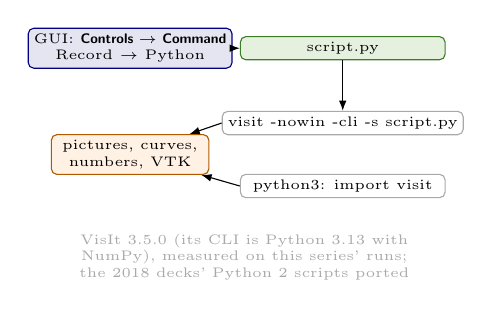
\begin{tikzpicture}[every node/.style={font=\tiny}, box/.style={draw, rounded corners=2pt, align=center, inner sep=2pt}]
  \node[box,draw=NavyBlue,fill=NavyBlue!10,minimum width=2.0cm] (gui) at (0,1.3) {GUI: \gui{Controls $\to$ Command}\\Record $\to$ Python};
  \node[box,draw=OliveGreen,fill=OliveGreen!10,minimum width=2.6cm] (s) at (2.7,1.3) {\code{script.py}};
  \node[box,draw=DarkGray,fill=white,minimum width=2.6cm] (cli) at (2.7,0.35) {\code{visit -nowin -cli -s script.py}};
  \node[box,draw=DarkGray,fill=white,minimum width=2.6cm] (py) at (2.7,-0.45) {\code{python3}: \code{import visit}};
  \node[box,draw=orange!70!black,fill=orange!10,minimum width=2.0cm] (out) at (0,-0.05) {pictures, curves,\\numbers, VTK};
  \draw[-{Latex[length=1.3mm]}] (gui) -- (s);
  \draw[-{Latex[length=1.3mm]}] (s) -- (cli);
  \draw[-{Latex[length=1.3mm]}] (cli.west) -- (out);
  \draw[-{Latex[length=1.3mm]}] (py.west) -- (out);
  \node[text=DarkGray,align=center,text width=4.9cm] at (1.45,-1.35) {VisIt 3.5.0 (its CLI is Python 3.13 with NumPy), measured on this series' runs; the 2018 decks' Python 2 scripts ported};
\end{tikzpicture}}
\end{frame}

% 2
\begin{frame}{Learning goals}
\label{fr:goals}
\footnotesize By the end of this chapter you should be able to:
\begin{itemize}
  \item Run VisIt's Python: interactively, from a script file with arguments, inside a running CLI, and from your own Python.
  \item Record what you do in the GUI as Python, and turn the recording into a script that loops over time.
  \item Find any function or attribute without a manual (\code{help}, \code{apropos}, \code{dir}, printing an attributes object).
  \item Check every step of a script (return values, \code{GetLastError()}), and know which failures VisIt does not report.
  \item Port a Python 2 VisIt script of the old decks to VisIt 3.5's Python 3.
  \item Combine VisIt with NumPy, inside VisIt's CLI or in your own Python.
\end{itemize}
\begin{punchbox}
\small Every new picture of a plot and every number of Part V was made by a script (the window screenshots are the old decks'). The GUI is where you design a picture; a script is how you make it again, for every frame and every run.
\end{punchbox}
\end{frame}

% 3
\begin{frame}{Where this chapter comes from}
\label{fr:sources}
\scriptsize
\begin{itemize}
  \item \al{``8 -- Visit from command line and Python''} (2018): ``Goal: Use visit for big data analysis without downloading the data or using the GUI'', on the Killdevil cluster: \code{module add visit/2.12.3}, \code{visit -cli -nowin} and \code{Source("heart\_script.py")}, or \code{visit -cli -nowin -s}; building VisIt with \code{build\_visit --mesa}; recording; a recorded script of IB/11's racetrack with a loop over time; and C. Strickland's ``Option 2: Run visit from python'': \code{import visit} into your own Python.
  \item \al{``6 -- Resampling AMR grids to Uniform Grid, exporting to .vtk, and recording in Python''} (2018), slides 2--4 and 15--16: ``record your python commands in visit 2.5.2''; ``Before you start doing anything, click on the execute button''; ``Then the code can be modified to loop through time.''
  \item \al{``3B -- Analyzing your IBFE simulation''} (2018), slides 3--8: record, edit the paths, add a loop, run on the cluster.
  \item \al{G. Hobson} (2020; chapter 31): \gui{Controls $\to$ Command}, \gui{Record}, \gui{Stop}, copy the code into ``a whitespace-sensitive text editor''.
  \item The decks point to Shannon Jones's video how-tos on recording (listed in chapter 0.1, not used here) and to a visitusers.org scripting tutorial (the site is gone).
\end{itemize}
\al{New here:} every claim run in VisIt 3.5.0 without a window, except those about the GUI (the Command window and its recorder: read from VisIt's source and GUI library and the 2018 recordings): the CLI's Python and packages, what functions return when they fail, what the recorder writes, the arguments a script receives, the external \code{import visit} route; and the scripts of chapters 27, 29--31 and 33 as worked examples.
\end{frame}

% 4
\begin{frame}{What changed since the 2018 decks}
\label{fr:old}
\scriptsize
\begin{tabular}{@{}L{0.38\textwidth}L{0.58\textwidth}@{}}
\toprule
2018 & VisIt 3.5.0 \\
\midrule
``VisIt's Python interpreter is \dots\ a basic Python 2.x environment \dots\ NumPy and matplotlib in particular are absent'' & the CLI is Python 3.13.9 with NumPy 2.3.4 and \code{visit\_utils}; matplotlib, SciPy and h5py are still absent (slide \ref{fr:numpy}) \\
Python 2's \code{print "..."}, integer \code{/}, \code{xrange} (the decks' own scripts use none of them) & Python 3: \code{print(...)}, \code{//} for integers, \code{range} (slide \ref{fr:py3}) \\
``click on the execute button'' to record & the button is \gui{Record} (\gui{Execute} runs the text of its tab; slide \ref{fr:record}) \\
Killdevil's \code{visit} module, VisIt 2.5.2 (``record your python commands in visit 2.5.2''), and \code{visit/2.12.3} & Puma's \code{visit/3.4.2} module or your own install (chapter 31); record in the version you will run \\
the Windows hotfix to \code{frontend.py} for \code{import visit} & not checked on Windows here; on Linux the route works with two environment variables (slide \ref{fr:import}) \\
\code{Source("script.py")} from the CLI prompt & still works; \code{-s script.py -- arguments} is easier to repeat \\
visitusers.org's tutorial & gone; the VisIt manual's Python chapter, and \code{help()} and \code{apropos()} in the CLI \\
\bottomrule
\end{tabular}
\sourcecredit{The 2018 decks of the previous slide; VisIt 3.5.0: \code{wsl/final/ch32\_*.sh}.}
\end{frame}

% 5
\begin{frame}[fragile]{Six ways to run VisIt's Python}
\label{fr:ways}
\begin{lstlisting}[style=shell]
visit -cli                                   # 1. a Python prompt with a VisIt window
visit -cli -nowin                            #    the same without a window: >>> OpenDatabase(...)
visit -nowin -cli -s script.py -- a b k=v    # 2. a script with arguments (the way of this series)
>>> Source("script.py")                      # 3. a script run inside a CLI that is already open
printf 'print(Version())\nexit()\n' | visit -cli -nowin      # 4. commands piped in: ">>> 3.5.0"
visit -movie -scriptfile movie.py ...        # 5. a script inside the movie maker (chapter 30)
python3 my_analysis.py                       # 6. your own Python, with "import visit" (slide on import visit)
\end{lstlisting}
\footnotesize
\begin{itemize}\setlength{\itemsep}{1pt}
  \item In the GUI, \gui{Controls $\to$ Command} gives a seventh: Python typed or recorded in a window, run with \gui{Execute} (slide \ref{fr:record}).
  \item Every CLI run leaves \code{visitlog.py} in the working folder: the commands it sent, a log of the session.
  \item A script run with \code{-s} should end in \code{sys.exit()}: without it the CLI goes on to its prompt and, started from a terminal, waits there. In a batch job (chapter 31) Slurm gives the script \code{/dev/null} as input, and with that input the CLI ended at its prompt at once. The exit status was 250 every time, after \code{sys.exit(0)} too: count what a script wrote instead.
\end{itemize}
\sourcecredit{VisIt 3.5.0 \code{visit -help}; \code{wsl/final/ch32\_cli\_helpers.sh}; the prompt and the exit status: \code{scratch/ch32/verify\_agent/v5\_runs.sh}, \code{v9\_exitcodes.sh}; Slurm's \code{sbatch} manual (\code{--input}).}
\end{frame}

% 6
\begin{frame}[fragile]{A script's arguments}
\label{fr:args}
\begin{lstlisting}[style=python]
import sys
print(sys.argv)
# visit -nowin -cli -s args.py -- a b k=v
#   ['args.py', '--', 'a', 'b', 'k=v']
# visit -nowin -cli -np 2 -s args.py -- a b k=v
#   ['args.py', '--', 'a', 'b', 'k=v', '-engineargs', '-l;mpirun;-np;2', '-launchengine', 'localhost']
\end{lstlisting}
\footnotesize
\begin{itemize}\setlength{\itemsep}{1pt}
  \item Everything after \code{--} is the script's; VisIt keeps the \code{--} itself in \code{sys.argv}.
  \item With a parallel engine VisIt appends its own options: stop reading at \code{-engineargs} (the scripts of \code{examples/analysis} do).
  \item The pattern of this series: positional arguments for the data and the output folder, \code{key=value} for options, the defaults and their meaning in the script's docstring, printed when the arguments are missing (next slide).
\end{itemize}
\sourcecredit{\code{wsl/final/ch31\_parallel.sh} (the CLI's command line with \code{-np}); \code{print(sys.argv)} run with and without \code{-np 2} (VisIt 3.5.0; \code{scratch/ch31/verify\_agent/v3\_cli.sh}, \code{scratch/ch32/verify\_agent/v5\_runs.sh}).}
\end{frame}

\begin{frame}[fragile]{Reading the arguments}
\label{fr:args2}
\footnotesize The argument lines of \code{examples/analysis/visit\_queries.py}; every VisIt script there has the same loop (\code{visit\_3d.py} and \code{resample\_export.py} take three positional arguments):
\begin{lstlisting}[style=python]
args = []
for a in sys.argv[1:]:
    if a in ("-engineargs", "-launchengine"):
        break
    if a != "--":
        args.append(a)
if len(args) < 2:
    print(__doc__); sys.exit(1)
DB, OUT = args[0], args[1]
opt = dict(a.split("=", 1) for a in args[2:])
\end{lstlisting}
\footnotesize Then \code{opt.get("lim", "auto")} (a key of \code{visit\_movie\_frames.py}) and the like give each option with its default; \code{\_\_doc\_\_} is the docstring at the top of the file, so the help a user sees is the one written there.
\end{frame}

% 7
\begin{frame}{Recording in the GUI}
\label{fr:record}
\footnotesize
\gui{Controls $\to$ Command . . .} opens the Command window, laid out in VisIt 3.5 as in 2018. Its \gui{Commands} box has \gui{Record}, \gui{Pause} and \gui{Stop}, \gui{Store commands in} (\gui{Active tab}, \gui{First empty tab} or \gui{Macros}) and \gui{Append commands to existing text}; below it are eight numbered tabs, each a text box with \gui{Execute}, \gui{Clear} and \gui{Make macro}, and a \gui{Macros} tab with \gui{Update macros} and \gui{Clear}.
\begin{enumerate}\setlength{\itemsep}{1pt}
  \item \gui{Record}, then make the picture in the GUI as usual; \gui{Stop}. The Python for every step appears in the active tab's box.
  \item Copy it into an editor (``a whitespace-sensitive text editor'', 2020; the 2018 deck: ``Cut and paste python to a text editor (but not the software text edit)'').
  \item Keep what you need, put the paths in variables, add a loop over time (slide \ref{fr:time}), save a picture per step.
  \item \gui{Execute} runs whatever is in its tab's box, recorded or typed: a quick way to test a few lines against the open session.
\end{enumerate}
\begin{punchbox}
\footnotesize The 2018 decks said ``Before you start doing anything, click on the execute button''. The button that records is \gui{Record}; \gui{Execute} runs the text. ``You may want to run through what you are going to do before recording, however, and then actually record when you know you can go through the procedure without mistakes'' still holds.
\end{punchbox}
\sourcecredit{Button and tab names from VisIt 3.5.0's GUI library (\code{wsl/final/ch32\_cmdwin\_strings.sh}), their layout from VisIt's \code{QvisCommandWindow.C} and the 2018 deck's screenshot (VisIt 2.13.0, slide 11); the 2018 decks; G. Hobson (2020), slides 6--7.}
\end{frame}

% 8
\begin{frame}[fragile]{What the recorder writes, and what to keep}
\label{fr:recorded}
\begin{columns}[T]
\column{0.5\textwidth}
\begin{lstlisting}[style=pytiny]
# recorded (2018, IB/11's racetrack; the paths shortened)
OpenDatabase("localhost:/.../4-VP_heart_viz_IB2d/lag_data.visit", 0)
OpenDatabase("localhost:/.../4-VP_heart_viz_IB2d/dumps.visit", 0)
AddPlot("Pseudocolor", "Omega", 1, 0)
DrawPlots()
ActivateDatabase("localhost:/.../4-VP_heart_viz_IB2d/lag_data.visit")
AddPlot("Mesh", "heart_peri_512_vertices", 1, 0)
AddPlot("Mesh", "heart_race_512_vertices", 1, 0)
AddPlot("Mesh", "heart_tube_512_vertices", 1, 0)
AddPlot("Mesh", "markers_512_vertices", 1, 0)
AddPlot("Mesh", "vp_aforce_512_vertices", 1, 0)
DrawPlots()
SaveWindowAtts = SaveWindowAttributes()
SaveWindowAtts.outputToCurrentDirectory = 0
SaveWindowAtts.outputDirectory = "./visit_images"
...                    # 15 more fields
SetSaveWindowAttributes(SaveWindowAtts)
SaveWindow()
\end{lstlisting}
\column{0.48\textwidth}
\scriptsize
\begin{itemize}\setlength{\itemsep}{1pt}
  \item \code{localhost:} and the absolute path of the machine it was recorded on: change the path (chapter 31); \code{localhost:} is the machine VisIt runs on and can stay (a \code{localhost:} path opened in 3.5.0).
  \item \code{AddPlot(type, variable, 1, 0)}: the two flags are \code{inheritSIL} and \code{applyOperators} (whether the new plot takes the active plot's SIL restriction, and its operators); \code{AddPlot(type, variable)} is enough.
  \item The recorder sets every field of an attributes object, including the defaults (the 2018 loop set 17 fields of \code{SaveWindowAttributes}). Keep the ones you changed; the rest only hides them.
  \item The zoom is recorded, and one of its lines must go: next slide.
  \item The Subset plot of \code{levels} that opening \code{dumps.visit} adds is not in the recording but is in the session: delete it in the script (chapter 30).
\end{itemize}
\end{columns}
\sourcecredit{``8 -- Visit from command line and Python'' (2018), slides 12--13; VisIt 3.5.0 \code{help(AddPlot)}; the \code{localhost:} path: \code{scratch/ch31/verify\_agent/v3\_cli.sh}.}
\end{frame}

\begin{frame}{The zoom in a recording}
\label{fr:zoom}
\footnotesize
\begin{itemize}\setlength{\itemsep}{2pt}
  \item The zoom is recorded. The zoom icon becomes \code{SetWindowMode("zoom")}; in a CLI without a window that line kills the viewer (``VisIt's viewer has terminated abnormally!''), and every later call fails (``VisIt's viewer is not running!'').
  \item The view the zoom gave is written as \code{View2DAtts} fields and \code{SetView2D(View2DAtts)} between \code{\# Begin spontaneous state} and \code{\# End spontaneous state}. Run without a window, such a block sets the view as it should.
  \item The 2020 deck: ``commands to do with spontaneous states \dots\ do not work on the cluster''. Delete the \code{SetWindowMode} lines; keep the view, or set it with numbers (\code{windowCoords}, chapter 30).
\end{itemize}
\sourcecredit{G. Hobson (2020), slide 13; VisIt's recorder (\code{Logging.C}: the spontaneous-state blocks, \code{SetWindowMode}) and viewer (\code{ViewerSubject.C}: the vis window's toolbar actions are passed to the recorder); \code{scratch/ch32/verify\_agent/t\_zoom.py}, \code{t1\_cli.py} (VisIt 3.5.0, no window).}
\end{frame}

% 9
\begin{frame}[fragile]{Finding your way without a manual (1/2): functions and plugins}
\label{fr:help}
\begin{lstlisting}[style=python]
>>> Version()                    # '3.5.0'
>>> apropos("lineout")           # functions whose name or help mentions it:
['ClearReferenceLines', 'GetGlobalLineoutAttributes', 'GetPlotInformation', 'Lineout', 'LineoutAttributes',
 'ResetLineoutColor', 'SetGlobalLineoutAttributes', 'SetWindowMode']
>>> help(Lineout)                # its synopsis, arguments, return value and an example
>>> PlotPlugins()                # ('Boundary', 'Contour', 'Curve', ... 'Vector', 'Volume'): 18 plots
>>> OperatorPlugins()            # ('AMRStitchCell', 'AxisAlignedSlice4D', 'BoundaryOp', 'Box', ...)
\end{lstlisting}
\footnotesize \code{apropos} searches the names and the help texts; \code{help} prints a function's synopsis, arguments, return value and example. Next: the attributes objects.
\sourcecredit{\code{wsl/final/ch32\_cli\_helpers.sh}, \code{ch32\_dir\_sliders.sh} (VisIt 3.5.0).}
\end{frame}

\begin{frame}[fragile]{Finding your way without a manual (2/2): attributes, metadata, plots}
\label{fr:help2}
\begin{lstlisting}[style=python]
>>> p = PseudocolorAttributes(); print(p)
scaling = Linear  # Linear, Log, Skew
skewFactor = 1
limitsMode = OriginalData  # OriginalData, ActualData
minFlag = 0
...
>>> md = GetMetaData("viz_IB2d/dumps.visit"); print(md.numStates, md.times[-1])
>>> ListPlots()                  # the plots of the window, with their databases and variables
>>> len([f for f in dir(p) if f[0] != "_"])    # 165 names: a Get and a Set for each of the 55 fields, and more
\end{lstlisting}
\footnotesize Printing an attributes object lists every field with its value and, for the choices, the names allowed (\code{p.Linear}, \code{p.Log}, \dots). That is the recorder's format, and the quickest documentation there is.
\sourcecredit{\code{wsl/final/ch32\_cli\_helpers.sh}, \code{ch32\_dir\_sliders.sh} (VisIt 3.5.0).}
\end{frame}

% 10
\begin{frame}[fragile]{The interface in one page}
\label{fr:api}
\scriptsize
\begin{tabular}{@{}L{0.18\textwidth}L{0.78\textwidth}@{}}
\toprule
task & functions (chapters where they, or their GUI counterparts, are used) \\
\midrule
data & \code{OpenDatabase}, \code{ActivateDatabase}, \code{CloseDatabase}, \code{ReplaceDatabase}, \code{GetMetaData} (26--31, 33) \\
plots & \code{AddPlot}, \code{DeleteAllPlots}, \code{SetActivePlots}, \code{HideActivePlots}, \code{DrawPlots}, \code{ListPlots} (26--31, 33) \\
attributes & \code{PseudocolorAttributes()}, \code{MeshAttributes()}, \code{VectorAttributes()}, \dots, \code{SetPlotOptions}; \code{BoxAttributes()}, \dots, \code{SetOperatorOptions} (26, 29) \\
operators & \code{AddOperator("Box")}, \code{"Slice"}, \code{"Resample"}, \code{"Displace"}, \code{"IntegralCurve"} (27--29, 31, 33) \\
expressions & \code{DefineScalarExpression}, \code{DefineVectorExpression} (26--29) \\
time & \code{TimeSliderGetNStates}, \code{SetTimeSliderState}, \code{GetTimeSliders}, \code{SetActiveTimeSlider}, \code{CreateDatabaseCorrelation} (26, 30) \\
view & \code{GetView2D}/\code{SetView2D} (\code{windowCoords}), \code{GetView3D}/\code{SetView3D} (27, 30) \\
annotation & \code{AnnotationAttributes()}, \code{SetAnnotationAttributes}, \code{CreateAnnotationObject("Text2D")} (26, 30) \\
saving & \code{SaveWindowAttributes()}, \code{SetSaveWindowAttributes}, \code{SaveWindow}; \code{ExportDatabase} (30, 33) \\
numbers & \code{Query}, \code{GetQueryOutputValue}, \code{QueryOverTime}, \code{Lineout}, \code{NodePick}, \code{GetPlotInformation} (29) \\
sessions & \code{SaveSession}, \code{RestoreSession} (26, 30) \\
\bottomrule
\end{tabular}
\end{frame}

\begin{frame}[fragile]{The pattern, and what this series does not call}
\label{fr:pattern}
\begin{lstlisting}[style=python]
p = PseudocolorAttributes()           # defaults; GetPlotOptions() would give the active plot's
p.colorTableName = CT; p.centering = p.Nodal
p.minFlag = 1; p.min = lo; p.maxFlag = 1; p.max = hi      # fixed limits
SetPlotOptions(p)                     # nothing changes on screen before this
\end{lstlisting}
\footnotesize
Pattern: make an attributes object (from its constructor for defaults, or \code{Get\dots()} for the current state), change fields, hand it back with \code{Set\dots()}. Nothing changes on screen until you do. No script of this series calls \code{CloseDatabase}, \code{ReplaceDatabase}, \code{HideActivePlots}, \code{CreateDatabaseCorrelation} or \code{RestoreSession} (\code{ListPlots} only on slide \ref{fr:help2}): their GUI counterparts are in chapter 26.
\sourcecredit{\code{examples/analysis/visit\_movie\_frames.py}, lines 99--101; \code{GetPlotOptions()}: \code{wsl/final/ch32\_getplotoptions.sh} (VisIt 3.5.0); the fact-check's search of chapters 26--33 and their scripts (\code{scratch/ch32/verify\_agent/api\_chapters.py}).}
\end{frame}

% 11
\begin{frame}[fragile]{Errors: what VisIt tells you, and what it does not}
\label{fr:errors}
\begin{lstlisting}[style=python]
r = OpenDatabase("/no/such/file.visit")    # prints "VisIt could not read from the file ...", returns 0
print(GetLastError())                      # the same message, as a string
r = OpenDatabase("viz_IB2d/dumps.visit")   # one that exists: returns 1
r = AddPlot("Pseudocolor", "NoSuchVariable")   # returns 0: "An invalid variable (NoSuchVariable) was specified."
r = DrawPlots()                            # returns 1 all the same
name = SaveWindow()                        # returns the file written: 'visit0000.png' (defaults: working folder)
\end{lstlisting}
\footnotesize
\begin{itemize}\setlength{\itemsep}{0pt}
  \item Most functions return 1 for success and 0 for failure; check the ones that matter (\code{OpenDatabase}, \code{AddPlot}) and stop the script, rather than draw nothing for an hour.
  \item \code{DrawPlots()} said 1 after a failed \code{AddPlot}: a return value is about that call only.
  \item Wrap the script in \code{try:} \dots\ \code{finally: sys.exit()} so that an exception ends the run instead of leaving the CLI waiting.
\end{itemize}
\sourcecredit{\code{wsl/final/ch32\_cli\_helpers.sh} (VisIt 3.5.0); the listing run as printed: \code{scratch/ch32/verify\_agent/t\_errors2.py}.}
\end{frame}

\begin{frame}{What VisIt does not report, and its logs}
\label{fr:silent}
\footnotesize
\begin{itemize}\setlength{\itemsep}{2pt}
  \item What VisIt does not report as an error (chapters 29--30): a missing output folder (``Saved'' and nothing written), a time query on a boxed plot 8\,\% low (the median; 25--31\,\% on frames of reversed flow), the Subset plot VisIt adds on opening drawing coloured lines, frames padded to 30 per second (at \code{-fps 10} a movie then shows 8.3 of your frames per second: 51 frames last 6.12 s). The CLI's exit status reports nothing either: 250 whatever happened (slide \ref{fr:ways}).
  \item \code{-debug 1} to \code{-debug 5} write logs of each VisIt process to the working folder (\code{A.cli.1.vlog}, \code{A.viewer.1.vlog}, \code{A.mdserver.1.vlog}, \code{A.engine\_ser.1.vlog}).
\end{itemize}
\sourcecredit{Chapters 29 and 30; \code{wsl/final/ch32\_cli\_helpers.sh}, \code{scratch/ch32/verify\_agent/v9\_exitcodes.sh} (VisIt 3.5.0).}
\end{frame}

% 12
\begin{frame}[fragile]{Time: the loop every script needs}
\label{fr:time}
\begin{columns}[T]
\column{0.55\textwidth}
\begin{lstlisting}[style=pytiny]
md = GetMetaData(DB)                  # times, cycles, variables
N = md.numStates
for k in range(N):                    # from dump 0
    for ts in GetTimeSliders():       # every slider
        SetActiveTimeSlider(ts)
        SetTimeSliderState(k)
    t = md.times[k]
    # ... a query, a picture, a lineout at time t
\end{lstlisting}
\column{0.43\textwidth}
\scriptsize
\begin{itemize}\setlength{\itemsep}{1pt}
  \item The 2018 loop (\code{TimeSliderNextState()} before the first save) skipped dump 0; this one does not (chapter 30).
  \item With two databases open VisIt has a slider for each and one for their correlation; setting only the active one leaves the others behind (chapter 30).
  \item \code{md.times} are the dumps' times (\code{0.0, 0.04, \dots, 2.0} for IB/11): write them next to every number.
  \item \code{help(GetTimeSliders)} says it returns a tuple of strings; 3.5.0 returns a dictionary, slider name to state. A loop over it gets the names, as here.
\end{itemize}
\end{columns}
\vspace{1mm}
\footnotesize The 2018 deck: ``Add a loop to go through all times and save an image'', with \code{k=1}, \code{N=2} and ``\#Note we advance in time to skip t=0''.
\sourcecredit{``8 -- Visit from command line and Python'' (2018), slide 13; the loop of \code{examples/analysis/visit\_movie\_frames.py}; \code{GetTimeSliders()}: \code{wsl/final/ch32\_dir\_sliders.sh} (VisIt 3.5.0).}
\end{frame}

% 13
\begin{frame}[fragile]{Python 2 scripts in VisIt 3}
\label{fr:py3}
\scriptsize
\begin{tabular}{@{}L{0.33\textwidth}L{0.33\textwidth}L{0.28\textwidth}@{}}
\toprule
Python 2 (VisIt 2.x to 3.1) & Python 3 (VisIt 3.2 on) & why \\
\midrule
\code{print "t =", t} & \code{print("t =", t)} & a function now \\
\code{n = N/2} with integers & \code{n = N // 2} & \code{/} always gives a float \\
\code{xrange(N)} & \code{range(N)} & \code{xrange} is gone \\
\code{"\%s" \% k} & \code{"\%s" \% k}, \code{f"\{k\}"} & both work; f-strings are new \\
\code{d.has\_key(k)} & \code{k in d} & \\
\code{except Exception, e:} & \code{except Exception as e:} & syntax \\
tabs and spaces mixed in a block & one or the other & Python 3 refuses the mix (\code{TabError}) \\
\bottomrule
\end{tabular}

\vspace{2mm}
\footnotesize
\begin{itemize}\setlength{\itemsep}{1pt}
  \item The 2018 and 2020 scripts that chapters 30--32 draw on contain nothing above that Python 3 refuses: they compile as Python 3 as they are, tab-indented loops included. Their VisIt functions all exist in 3.5.0 (24 checked), and so do their attribute fields (about 100), except three names of the 2020 Vector plot's: the field \code{lineStyle} and its value \code{SOLID} are gone, and \code{colorByMag} is now \code{colorByMagnitude}; setting \code{colorByMag} stops the script (``NameError: name 'colorByMag' is not defined''). \code{print} an object to see its current fields.
  \item VisIt's \code{-py2to3} option (``Enable limited on-the-fly Python 2 to 3 conversion support'', \code{visit -help}) can run some old scripts unchanged; converting them is better.
\end{itemize}
\sourcecredit{VisIt 3.5.0 \code{visit -help}; \code{wsl/final/ch32\_api\_check.sh}, \code{ch32\_vector\_fields.sh}; the ports in \code{examples/analysis} (chapters 29--33).}
\end{frame}

% 14
\begin{frame}[fragile]{NumPy inside VisIt's CLI}
\label{fr:numpy}
\begin{lstlisting}[style=python]
import numpy as np                              # in VisIt 3.5.0's CLI: Python 3.13.9, NumPy 2.3.4
DefineScalarExpression("U_x", "U[0]")
AddPlot("Pseudocolor", "U_x"); DrawPlots(); SetTimeSliderState(40)       # IB/11, t = 1.6 s
Lineout(start_point=(0, 0.10, 0), end_point=(0, 0.20, 0), use_sampling=1, num_samples=50)
SetActiveWindow(2)                              # the lineout's curve window
xy = np.array(GetPlotInformation()["Curve"]).reshape(-1, 2)    # 51 (distance, U_x) pairs
q = np.trapezoid(xy[:, 1], xy[:, 0])            # 5.712e-3 m^2/s across the top vessel (chapter 29's averages.csv, t = 1.6)
\end{lstlisting}
\footnotesize
\begin{itemize}\setlength{\itemsep}{1pt}
  \item The 2018 deck said VisIt's Python was ``a basic Python 2.x environment \dots\ NumPy and matplotlib in particular are absent''. VisIt 3.5.0's CLI imports \code{numpy} (2.3.4), \code{vtk} (9.5.0), \code{PIL} (Pillow 12.0.0) and \code{visit\_utils}; \code{matplotlib}, \code{scipy}, \code{h5py}, \code{netCDF4}, \code{pyvista} and \code{pandas} are absent.
  \item Without \code{use\_sampling=1} the lineout samples where the line meets the mesh (52 points here, 5.709e-3).
  \item So arithmetic on VisIt's numbers can stay in the script (NumPy's \code{polyfit} and \code{linalg.lstsq} too); plots and SciPy's fits go outside: write CSV or \code{.curve} files and read them in your own Python (chapter 29's \code{read\_curve.py}), or use the next slide's route.
  \item Do not \code{pip install} into VisIt's Python; keep VisIt's install as it came.
\end{itemize}
\sourcecredit{\code{wsl/final/ch32\_syspython2.sh}, \code{ch32\_numpy\_lineout.sh}, \code{ch32\_api\_check.sh}, \code{visit\_py\_pkgs.sh} (VisIt 3.5.0, Linux); the calls as in \code{examples/analysis/visit\_queries.py}.}
\end{frame}

% 15
\begin{frame}[fragile]{VisIt inside your own Python}
\label{fr:import}
\begin{lstlisting}[style=shell]
export PATH=/opt/visit/bin:$PATH                                  # `visit` must be found
export LD_LIBRARY_PATH=/opt/visit/3.5.0/linux-x86_64/lib          # its libraries too
python3 my_analysis.py
\end{lstlisting}
\begin{lstlisting}[style=python]
import sys
import matplotlib.pyplot as plt              # your Python's packages, in the same script: import them before visit
sys.path.append("/opt/visit/3.5.0/linux-x86_64/lib/site-packages")
import visit
visit.LaunchNowin()                          # or visit.AddArgument("-nowin"); visit.Launch()
visit.OpenDatabase("viz_IB2d/dumps.visit")
visit.AddPlot("Pseudocolor", "Omega"); visit.DrawPlots(); visit.SetTimeSliderState(50)
visit.Query("MinMax"); print(visit.GetQueryOutputValue())   # (-396.98..., 412.50...), as in the CLI
\end{lstlisting}
\footnotesize
\begin{itemize}\setlength{\itemsep}{1pt}
  \item The functions are the CLI's, prefixed by \code{visit.}. The 2018 Windows hotfix to \code{frontend.py} was not tried.
  \item Why the two variables, and what happened when this ran: next slide.
\end{itemize}
\sourcecredit{``8 -- Visit from command line and Python'' (2018), slides 15--18; \code{wsl/final/ch32\_syspython*.sh} (paths shortened to \code{/opt/visit}).}
\end{frame}

\begin{frame}{VisIt inside your own Python: what was measured}
\label{fr:import2}
\footnotesize
\begin{itemize}\setlength{\itemsep}{2pt}
  \item C. Strickland's route of 2018, measured with Ubuntu's Python 3.12: without \code{LD\_LIBRARY\_PATH}, \code{import visit} stops with ``ImportError: libviewerproxy.so: cannot open shared object file''; without VisIt's \code{bin} on the \code{PATH}, \code{LaunchNowin()} with ``Unable to launch program visit''. With both it ran and gave the same MinMax every time, in a few runs after a harmless \code{BrokenPipeError} traceback from VisIt's launcher.
  \item Python then often aborted on exit, after the script's last line (``Aborted (core dumped)'', status 134): in 12 of 18 runs with matplotlib imported after \code{visit}, 1 of 9 with it imported first (as on the previous slide), none of 10 with neither matplotlib nor NumPy. The output was complete every time; the exit status cannot be trusted.
  \item \code{export LD\_LIBRARY\_PATH=\dots} holds for every program started from that shell afterwards, and system programs then load VisIt's own copies of their libraries. \code{LD\_LIBRARY\_PATH=\dots\ python3 my\_analysis.py} sets it for that one command (whether that changes the abort on exit was not tested).
\end{itemize}
\sourcecredit{\code{wsl/final/ch32\_syspython*.sh}; \code{scratch/ch32/verify\_agent/v5\_runs.sh}, \code{v6\_import.sh}, \code{v7\_import\_repeat.sh}, \code{v7b\_import\_repeat.sh} (Ubuntu 24.04's \code{python3} 3.12.3, VisIt 3.5.0).}
\end{frame}

% 16
\begin{frame}{Many runs: one script, a loop outside}
\label{fr:sweep}
\footnotesize
A parameter sweep (chapter 3; IB/01's job array) leaves one folder per run (\code{run\_1}, \code{run\_2}, \dots). Run the same VisIt script on each:
\begin{itemize}\setlength{\itemsep}{1pt}
  \item \al{A shell loop}: \code{for d in run\_*; do visit -nowin -cli -s visit\_queries.py -- \$d/viz\_IB2d/dumps.visit \$d/analysis; done}. Each run gets a fresh VisIt; a failure stops one run, not the sweep. Give \code{box=}, \code{point=} and \code{line=} for your geometry: the defaults are IB/11's top vessel, and on another run they measure nothing meaningful, without an error.
  \item \al{A Slurm array}: one array task per run folder, the same script (chapter 31's batch job, with \code{\$SLURM\_ARRAY\_TASK\_ID} choosing the folder as in IB/01's \code{job\_array.slurm}, chapter 3).
  \item \al{One VisIt for all}: \code{CloseDatabase} and \code{OpenDatabase} (or \code{ReplaceDatabase}, which keeps the plots) inside one script. Fewer start-ups (VisIt takes a few seconds to start), but one error ends everything.
  \item Write each run's numbers to its own folder (\code{averages.csv}, \code{frames.csv}), then gather them in Python or MATLAB: the record of chapter 29 (protocol, data sheet, report).
\end{itemize}
\begin{punchbox}
\footnotesize Test on one run, then on two, then on all; and count the outputs (frames, rows) of every run, not only of the first.
\end{punchbox}
\end{frame}

% 17
\begin{frame}{The scripts of this series, as examples}
\label{fr:examples}
\scriptsize
\begin{tabular}{@{}L{0.25\textwidth}L{0.5\textwidth}L{0.17\textwidth}@{}}
\toprule
\code{examples/analysis/} & what it shows & chapter \\
\midrule
\code{visit\_movie\_frames.py} & arguments, the structure's meshes found from the metadata, fixed limits from a query, a Text2D time stamp, a loop over time, a CSV of what was written, \code{first=} to number a later chunk on (chapter 31) & 30 \\
\code{visit\_queries.py} & a Box, queries frame by frame and through time, a node pick through time, lineouts, curves saved as \code{.curve} files and their values read from the plots, an expression for the normal velocity & 29 \\
\code{visit\_3d.py} & 3D views by numbers, slices, isosurfaces, vectors on a slice, expressions & 27 \\
\code{resample\_export.py} & the Resample operator and \code{ExportDatabase} in a loop, and a fix for an export quirk & 33 \\
\code{visit\_frames.slurm} & the CLI in a batch job & 31 \\
\code{make\_movie.py}, \code{read\_curve.py} & plain Python on VisIt's outputs: ffmpeg, \code{.curve} files & 30, 29 \\
\bottomrule
\end{tabular}

\vspace{2mm}
\footnotesize Each Python script starts with a docstring that says how to run it and what it writes (the Slurm script, with comments). The VisIt ones print what they are doing (flushed, so a batch log shows it) and end with \code{sys.exit()}, inside \code{try}/\code{finally} in \code{visit\_movie\_frames.py} and \code{visit\_queries.py}. All were run on this series' data before they were published (\code{visit\_frames.slurm} with bash on this computer, not yet on Puma: chapter 31).
\end{frame}

% 18
\begin{frame}{When a script goes wrong}
\label{fr:trouble}
\scriptsize
\begin{tabular}{@{}L{0.42\textwidth}L{0.53\textwidth}@{}}
\toprule
what you see & what to do \\
\midrule
the CLI waits at \code{>>>} after the script (started from a terminal; a batch job's input is \code{/dev/null}) & end it with \code{sys.exit()}, inside \code{finally:} \\
\code{SyntaxError} on \code{print "\dots"} & a Python 2 script: slide \ref{fr:py3} \\
\code{TabError} or \code{IndentationError} & tabs mixed with spaces (recorded code pasted into an editor) \\
\code{ValueError} reading \code{key=value} arguments & \code{-np} added \code{-engineargs}: slide \ref{fr:args} \\
nothing drawn, and the script ran on & a failed \code{AddPlot} earlier (its message is in the log): check its return value, \code{GetLastError()} \\
``An invalid variable'' & the variable's name in this database: \code{GetMetaData}; IBAMR 0.19 writes \code{U}, not \code{U\_x} (chapter 26) \\
the recorded path does not open & another machine's path (the \code{localhost:} before it can stay; slide \ref{fr:recorded}) \\
a picture of the whole domain & the script never sets the view: keep the recorded \code{SetView2D} (slide \ref{fr:zoom}), or set \code{windowCoords} \\
``VisIt's viewer has terminated abnormally!'' & a recorded \code{SetWindowMode("zoom")}: delete it (slide \ref{fr:zoom}) \\
\code{ImportError: libviewerproxy.so} in your Python & \code{LD\_LIBRARY\_PATH} (slide \ref{fr:import}) \\
\code{ModuleNotFoundError} for \code{matplotlib} in the CLI & not in VisIt's Python: write the numbers out, or use your own Python \\
\bottomrule
\end{tabular}
\end{frame}

% 19
\begin{frame}{Exercises}
\label{fr:exercises}
\footnotesize
\begin{enumerate}\setlength{\itemsep}{1pt}
  \item Record a picture of IB/11's vorticity in the GUI (\gui{Record}, \gui{Stop}); cut the recording down to the lines that matter; run it with \code{visit -nowin -cli -s} and compare the pictures.
  \item Add a loop over time that writes one picture per dump, numbered without gaps, and a CSV of the times.
  \item Use \code{apropos} and \code{help} to find how to save a curve window as a \code{.curve} file; do it.
  \item Port one of the 2018 or 2020 scripts quoted in chapters 31--32 to VisIt 3.5 (paths, dump 0, the renamed fields of slide \ref{fr:py3}; their syntax is already Python 3).
  \item Compute the flow rate across a line with NumPy inside the CLI, and check it against chapter 29's number (its \code{averages.csv}: $5.712\times10^{-3}$ m$^2$/s at $t = 1.6$ s).
  \item Run the same analysis from your own Python with \code{import visit}, and plot the result with matplotlib in the same script.
  \item Run \code{visit\_queries.py} on every run of a small sweep with a shell loop; gather the results in one table.
\end{enumerate}
\end{frame}

% 20
\begin{frame}{Summary}
\label{fr:summary}
\footnotesize
\begin{itemize}\setlength{\itemsep}{1pt}
  \item \code{visit -nowin -cli -s script.py -- arguments} is the way to repeat anything; the GUI's \gui{Record} writes the first draft.
  \item VisIt 3.5's CLI is Python 3.13 with NumPy; old scripts may need Python 3 syntax (the decks' own do not), need new paths, and should save dump 0.
  \item \code{help}, \code{apropos}, \code{print(attributes)}, \code{GetMetaData}, \code{ListPlots}: the documentation inside VisIt.
  \item Check return values and \code{GetLastError()}; some failures are silent, so count what a script writes.
  \item Your own Python can drive VisIt with \code{import visit}, given VisIt's \code{bin} on the \code{PATH} and its \code{lib} on \code{LD\_LIBRARY\_PATH}.
\end{itemize}
\begin{punchbox}
\small A script is the record of how a picture or a number was made. Keep it with the run.
\end{punchbox}
\end{frame}

% 21
\begin{frame}{References and credits}
\label{fr:refs}
\scriptsize
\begin{itemize}
  \item L.\,A. Miller, ``8 -- Visit from command line and Python'' (2018; with C. Strickland's notes on controlling VisIt from Python), ``6 -- Resampling AMR grids to Uniform Grid, exporting to .vtk, and recording in Python'' (2018), ``3B -- Analyzing your IBFE simulation'' (2018).
  \item G. Hobson, ``Post-Processing IBAMR Simulation Data in VisIt on a Computing Cluster'' (2020), slides 6--7 and 13.
  \item VisIt 3.5.0, \url{https://visit-dav.github.io/visit-website/}; its user manual's chapter on the Python interface, \url{https://visit-sphinx-github-user-manual.readthedocs.io/}; H. Childs et al., ``VisIt: An end-user tool for visualizing and analyzing very large data'', in \emph{High Performance Visualization}, CRC Press (2012) 357--372.
  \item The runs: IB/11 (\code{TARGET\_VP}), IBAMR 0.19.0; the measurements \code{wsl/final/ch32\_*.sh} in the working folder.
\end{itemize}
\end{frame}

\end{document}
